\documentclass{article}

% Language setting
% Replace `english' with e.g. `spanish' to change the document language
\usepackage[spanish]{babel}

% Set page size and margins
% Replace `letterpaper' with `a4paper' for UK/EU standard size
\usepackage[letterpaper,top=2cm,bottom=2cm,left=3cm,right=3cm,marginparwidth=1.75cm]{geometry}

% Useful packages
\usepackage{amsmath}
\usepackage{graphicx}
\usepackage{enumitem}
\usepackage{comment}
\usepackage{wrapfig}
\usepackage[colorlinks=true, allcolors=blue]{hyperref}

\title{Matemática Discreta Tema 1. Algoritmos y números}
\author{Martín González Dios 
\href{https://github.com/martindios}{\includegraphics[height=0.5cm]{github.png}}}

\begin{document}
\maketitle

\section{Algoritmos}
Un algoritmo es una \textbf{sucesión finita de instrucciones precisas} (pasos sucesivos definidos) para realizar una tarea que \textbf{tiene un final}. Sus propiedades principales son:
\begin{itemize}
    \item Tiene una \textbf{entrada} (input) y produce una \textbf{salida} (output y solución) correcta en un tiempo.
    \item Tiene un \textbf{propósito} concreto.
    \item Los pasos están definidos con \textbf{precisión}.
    \item Se aplica a todos los problemas (\textbf{generalidad}).
    \item Es \textbf{efectivo}, realizando cada paso con exactitud y en un tiempo finito.
    \item Es \textbf{eficiente}, se ejecuta en un tiempo polinómico.
\end{itemize}

\subsection{Algoritmos de búsqueda}
Estos algoritmos \textbf{localizan un elemento} (x) en una lista ordenada de elementos. La solución es la ubicación del elemento (x) en la lista o la declaración de que no está en ella.
\begin{itemize}
    \item \textbf{Búsqueda lineal o secuencial} (lista ordenada): compara x con $a_0$, si x = $a_0$ la salida es 0, si no, se compara con el siguiente ($a_1$, $a_2$, $a_3$, ...) hasta encontrar una coincidencia. Si no se encuentra la solución es false.
    \item \textbf{Búsqueda binaria} (lista creciente): compara x con el elemento central de la lista (si hay un número par de elementos elegimos m = $\lfloor n/2 \rfloor$), dividiéndola por ese término, que se incluye en la primera lista y restringiendo la búsqueda a la primera o segunda mitad de la lista (depende de si x es mayor o menor que el elemento central). Se repite el proceso en la sublista correspondiente (que tiene como mucho $\lceil (n+1)/2 \rceil$ elementos) hasta obtener un único elemento (que puede ser x o no encontrarse en la lista). (n es la posición del elemento, que empieza en 0)
\end{itemize}

\subsection{Funciones enteras}
\begin{itemize}
    \item Suelo, parte entera o \textbf{floor}: $\lfloor x \rfloor$ es el mayor entero tal que $z \leq x$. \\
    $\lfloor 3/2 \rfloor$ = $\lfloor 1.5 \rfloor$ = 1
    \item Techo o \textbf{ceiling}: $\lceil x \rceil$ es el menor entero tal que $z \geq x$. \\
    $\lceil 3/2 \rceil$ = $\lceil 1.5 \rceil$ = 2
    
\end{itemize}

\newpage

\section{Notación Big-$\mathcal{O}$}

\begin{wrapfigure}[]{r}{0.35\linewidth}
    \centering
    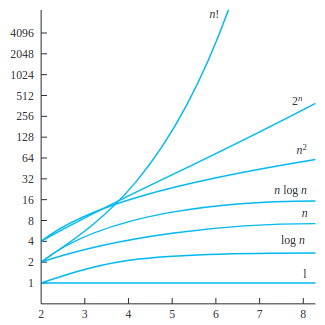
\includegraphics[width=\linewidth]{img-t1/img_036_28.png}
    \caption{Gráfica de funciones de crecimiento más usadas en Big-$\mathcal{O}$}
\end{wrapfigure}

Sea f y g funciones del conjunto de los enteros o del conjunto de los números reales al conjunto de los números reales. Decimos que $f(x)$ es $\mathcal{O}(g(x))$ si existen constantes C y k tales que $|f(x)| \leq C|g(x)|$ siempre que x $>$ k. [Esto se lee como "$f(x)$ es big-o de $g(x)$"]. \\

Observación: intuitivamente, la definición de que $f(x)$ es $\mathcal{O}(g(x))$ dice que $f(x)$ \textbf{crece más lentamente que algún múltiplo fijo} de $g(x)$ a medida que x crece sin límite. \\

Las constantes \textbf{C y k} de la definición se llaman \textbf{testigos de la relación} $f(x)$ es $\mathcal{O}(g(x))$. Para establecer que $f(x)$ es $\mathcal{O}(g(x))$ necesitamos solo un par de testigos para esta relación. Es decir, para demostrar que $f(x)$ es $\mathcal{O}(g(x))$ solo necesitamos encontrar un par de constantes C y k, los testigos, tales que $|f(x)| \leq C|g(x)|$ siempre que x $>$ k. \\

Cabe destacar que cuando hay un par de testigos para la relación $f(x)$ es $\mathcal{O}(g(x))$, hay infinitos pares de testigos. \\

\subsection{Reglas de notación Big-$\mathcal{O}$}
\begin{itemize}
    \item Si $f_1(x)$ es $\mathcal{O}(g_1(x))$ y $f_2(x)$ es $\mathcal{O}(g_2(x))$ $\xrightarrow{}$ $(f_1+f_2)(x)$ es $\mathcal{O}(max\{|g_1(x)|, |g_2(x)|\})$ \\
    Si $f_1(x)$ y $f_2(x)$ es $\mathcal{O}(g(x))$ $\xrightarrow{}$ $(f_1+f_2)(x)$ es $\mathcal{O}(g(x))$
    
    \item Si $f_1(x)$ es $\mathcal{O}(g_1(x))$ y $f_2(x)$ es $\mathcal{O}(g_2(x))$ $\xrightarrow{}$ $(f_1*f_2)(x)$ es $\mathcal{O}(g_1(x)*g_2(x))$

    \item Si $f(x)$ es $\mathcal{O}(g(x))$ y $g(x)$ es $\mathcal{O}(h(x))$ $\xrightarrow{}$ $f(x)$ es $\mathcal{O}(h(x))$

    \item Si $f(x)$ es $\mathcal{O}(g(x))$ $\xrightarrow{}$ $a*f(x)$ es $\mathcal{O}(g(x))$ para cualquier a
\end{itemize}

\subsection{Ejemplo 1}
$f(x) = x^{2}+2x+1$ es $\mathcal{O}(x^2)$. \textbf{Sea $f(x)$ un polinomio de grado n $\xrightarrow{}$ $f(x)$ es $\mathcal{O}(x^n)$} 

\subsection{Ejemplo 2}
Explicar que $7x^2$ es $\mathcal{O}(x^3)$. Cuando x $>$ 7 tenemos que $7x^2$ $<$ $x^3$ (obteniendo esta inecuación multiplicando los dos lados de x $>$ 7 por $x^2$). Consecuentemente, podemos tomar C = 1 y k = 7 como testigos de la relación $7x^2$ es $\mathcal{O}(x^3)$.  

\newpage

\subsection{Ejemplo 3}
n $<$ $2^n$ con cualquier n entero positivo. Explicar que esta inecuación implica que n es $\mathcal{O}(2^n)$ y usar esta inecuación para demostrar que log(n) es $\mathcal{O}(n)$. \\

Usando la inecuación n $<$ $2^n$ concluimos que n es $\mathcal{O}(2^n)$ tomando k = C = 1. Nótese que, dado que la función del logaritmo es creciente, al tomar logaritmos (base 2) a ambos lados de esta igualdad se muestra que: log(n) $<$ n (Tomando nuevamente k = C = 1 como testigos). $log(n)$ es $\mathcal{O}(n)$\\

\textbf{Si tuviésemos logaritmos en base b, donde b es diferente de 2, seguiríamos teniendo que $log_b(n)$ es $\mathcal{O}(n)$ con cualquier n positivo entero.} (si está elevado a un c positivo daría igual, sigue siendo $\mathcal{O}(n)$). \\
($log_b(n)^c$ es $\mathcal{O}(n^d)$ siendo d el grado del polinomio de la función $f(x)$)

\subsection{Ejemplo 4}
Estimar el Big-$\mathcal{O}$ para $f(n)=3nlog(n!)+(n^2+3)log(n)$, donde n es un positivo entero. \\

En primer lugar se estima $3nlog(n!)$. Sabemos que n! $\leq$ $n^n$: log(n!) $\leq$ log($n^n$) = n*log(n), por lo tanto log(n!) es $\mathcal{O}(nlog(n))$. 3n es $\mathcal{O}(n)$. Entonces  $3n*log(n!)$ es $\mathcal{O}(nlog(n))$. \\

El siguiente producto a estimar es $(n^2+3)log(n)$. $n^2+3$ es $\mathcal{O}(n^2)$. Por lo tanto, $(n^2+3)log(n)$ es $\mathcal{O}(n^2log(n))$. \\

Combinando las soluciones $f(n)=3nlog(n!)+(n^2+3)log(n)$ es $\mathcal{O}(n^2log(n))$.

\section{Notación Big-$\Omega$ y Big-$\Theta$}

\subsection{Big-$\Omega$}
Sea f y g funciones del conjunto de enteros o del conjunto de los números reales al conjunto de los números reales. Decimos que $f(x)$ es $\Omega(g(x))$ si hay constantes positivas C y k tales que $|f(x)| \geq  C|g(x)|$ para cualquier x $>$ k. [Se lee como "f(x) es big-omega de g(x)" o "f(x) es del orden al menos de g(x)"]. \\

Hay una fuerte relación entre big-$\mathcal{O}$ y big-$\Omega$, \textbf{de hecho $f(x)$ es $\Omega$(g(x)) si y solo si $g(x)$ es $\mathcal{O}$($f(x)$).} \\

\subsection{Big-$\Theta$}
Sea f y g funciones del conjunto de enteros o del conjunto de los números reales al conjunto de los números reales. Decimos que $f(x)$ es $\Theta(g(x))$ si f(x) es $\mathcal{O}(g(x))$ y f(x) es $\Omega(g(x))$. [Se lee como "f(x) es big-theta de g(x)" o "f(x) es del orden de g(x)"] \\

Cuando $f(x)$ es $\Theta(g(x))$ también es el caso de que $g(x)$ es $\Theta(f(x))$.

\subsection{Ejemplo 1}
Explica que $3x^2+8xlog(x)$ es $\Theta(x^2)$. \\

Porque $0 \leq 8xlog(x) \leq 8x^2$, lo que sigue que $3x^2+8xlog(x) \leq 11x^2$ para x $>$ 1. Consecuentemente, $3x^2+8xlog(x)$ es $\mathcal{O}(x^2)$, y claramente $x^2$ es $\mathcal{O}(3x^2+8xlog(x))$. \\

\textbf{El término mayor de un polinomio determina su orden. Por ejemplo, si $f(x) = 3x^5+x^4+17x^3+2$, por lo tanto $f(x)$ es del orden de $x^5$.}

\newpage

\section{Complejidad de un algoritmo}

\begin{wrapfigure}[]{r}{0.45\linewidth}
    \centering
    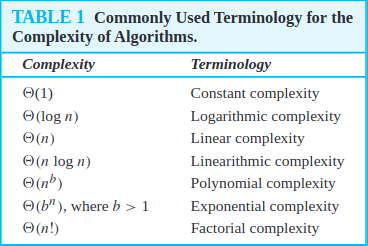
\includegraphics[width=\linewidth]{img-t1/img_951_53.png}
    \caption{Terminología para la complejidad algorítmica}
\end{wrapfigure}

Un algoritmo debe producir siempre la respuesta correcta y ser eficiente en términos de tiempo y espacio. La eficiencia se mide a través de la \textbf{complejidad temporal}, que se refiere al número de operaciones necesarias para resolver un problema de un tamaño específico, y la complejidad espacial, que se relaciona con la memoria requerida. \\

\textbf{La complejidad temporal se expresa en función del número de operaciones básicas} (como suma, multiplicación y comparación) en lugar de en tiempo real, debido a las variaciones en la velocidad de diferentes computadoras. 

\subsection{Ejemplo 1}

Describe la \textbf{complejidad temporal del algoritmo de búsqueda lineal}.

\begin{figure}[h]
    \centering
    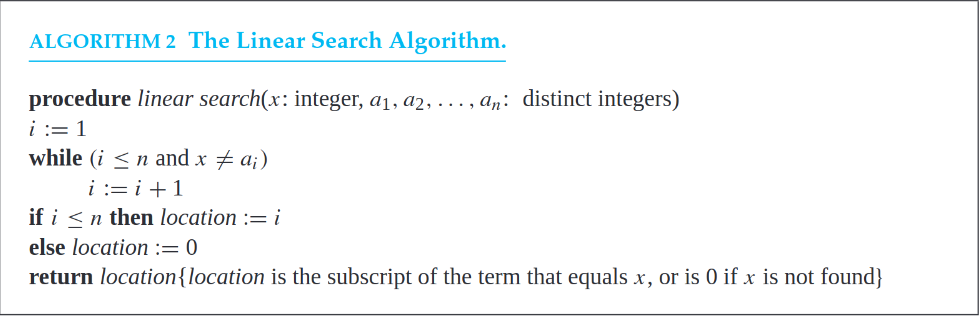
\includegraphics[width=0.7\textwidth]{img-t1/img_408_18.png}
\end{figure}

En cada paso del bucle del algoritmo, se realizan 2 comparaciones: una i $\leq$ n, para ver si se ha alcanzado el final de la lista, y una x $\leq$ $a_i$, para comparar el elemento x con un término de la lista. Finalmente, se realiza una comparación más i $\leq$ n fuera del bucle. En consecuencia, si x = $a_i$, se utilizan 2i + 1 comparaciones. Se requieren más comparaciones, \textbf{2n + 2, cuando el elemento no está en la lista}. En este caso, se utilizan 2n comparaciones para determinar que x no es $a_i$, para i = 1, 2, ..., n, se utiliza una comparación adicional para salir del bucle, y se realiza una comparación fuera del bucle. Por lo tanto, cuando x no está en la lista, se utilizan un total de 2n + 2 comparaciones. Así, una búsqueda lineal requiere $\Theta(n)$ comparaciones en el peor de los casos, porque 2n + 2 es $\Theta(n)$.

\newpage

\subsection{Ejemplo 2}
¿Cuál es el peor caso de \textbf{complejidad del bubble sort} en términos de número de comparaciones hechas?

\begin{figure}[h]
    \centering
    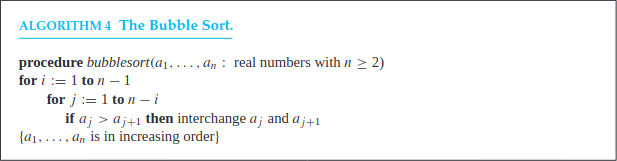
\includegraphics[width=0.7\textwidth]{img-t1/img_603_44.png}
\end{figure}

El bubble sort ordena la lista mediante una secuencia de pasadas a través de la lista. Durante cada iteración el algoritmo compara sucesivamente los elementos adyacentes, intercambiándolos si es necesario. Cuando \textbf{la i-ésima iteración} empieza, se garantiza que los i - 1 elementos más grandes están en las posiciones correctas. Durante esta iteración se utilizan \textbf{n - 1 comparaciones}. En consecuencia, el número total de comparaciones utilizadas por el ordenamiento burbuja para ordenar una lista de n elementos es \textbf{(n-1)+(n-1)+...+2+1}=$\frac{(n-1)n}{2}$.
Cabe destacar que el bubble sort siempre hace muchas comparaciones, ya que continúa aunque la lista esté completamente ordenada en un paso intermedio. Por lo tanto, el bubble sort utiliza (n-1)n/2 comparaciones, por lo que es $\Theta(n^2)$ en el peor caso de complejidad en términos de número de comparaciones usado.

\subsection{Ejemplo 3}
¿Cuántas \textbf{sumas y multiplicaciones} de enteros son usadas en el algoritmo de \textbf{multiplicación matricial} para multiplicar dos n x n matrices con entradas enteras?

\begin{figure}[h]
    \centering
    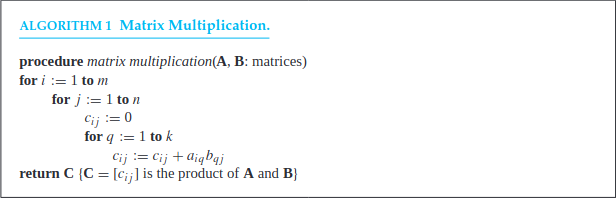
\includegraphics[width=0.65\textwidth]{img-t1/img_031_03.png}
\end{figure}

Hay $n^2$ entradas en el producto de A y B. Para encontrar cada entrada es necesario un total de n multiplicaciones y n - 1 sumas. Así, un \textbf{total de $n^3$ multiplicaciones y $n^2(n-1)$ sumas son usadas}.

\newpage

\section{Aritmética entera}

\subsection{División}
Si $a$ y $b$ son enteros con $a$ $\neq$ 0, decimos que $a$ divide a $b$ si hay \textbf{un entero $c$ tal que $b$ = $ab$}, o equivalentemente, que $\frac{a}{b}$ es un entero. Cuando $a$ divide a $b$ decimos que $a$ es un factor de $a$ y $b$ es un múltiplo de $a$. La notación $a$ $|$ $b$ denota que $a$ divide a $b$. Escribimos $a$ $\not|$ $b$ cuando $a$ no divide a $b$. \\

Teniendo $n$ y $d$ positivos enteros, ¿\textbf{cuántos positivos enteros que no excedan $n$ son divisibles entre $d$}?\\
Los positivos enteros divisibles por $d$ son todos los enteros de la forma $dk$, donde $k$ es un positivo entero. Así, el número de positivos enteros divisibles por $d$ que no exceda $n$ es igual al número de enteros $k$ con 0 $<$ $dk$ $\leq$ $n$, o con 0 $<$ $k$ $\leq$ $n/d$. Por lo tanto, \textbf{hay $\lfloor n/d \rfloor$ positivos que no excedan $n$ y sean divisibles entre $d$}. \\

\textbf{Sea $a$, $b$ y $c$ enteros, donde $a$ $\neq$ 0:}
\begin{itemize}
    \item Si $a$ $|$ $b$ y $a$ $|$ $c$, entonces $a$ $|$ $(b+c)$.
    \item Si $a$ $|$ $b$, entonces $a$ $|$ $bc$ para todos los enteros $c$.
    \item Si $a$ $|$ $b$ y $b$ $|$ $c$, entonces $a$ $|$ $c$.
    \item Si $a$ $|$ $b$ y $a$ $|$ $c$, entonces $a$ $|$ $mb + nc$ con cualquier n y m enteros.
\end{itemize}

El \textbf{algoritmo de la división}: \\
Sea $a$ un entero y $d$ un positivo entero. Entonces hay unos únicos enteros $q$ y $r$, con 0 $\leq$ $r$ $<$ $d$, tal que $a$ = $dq$ + $r$. 

\subsection{Números primos}
Un entero $p$ mayor que 1 es llamado primo si los únicos divisores positivos son 1 y $p$. Un número positivo que no sea primo se le llama compuesto. \\

(\textbf{Teorema de Euclides}: existen infinitos primos. \textbf{Primos de Mersenne}: $2^p$ - 1 con p primo, son primos [falso para p = 11 por ejemplo]) \\

\textbf{Teorema fundamental de la aritmética}: \\
Todo entero positivo $>$ 1 se puede factorizar (descomponer) de manera única como un primo o un producto de números primos donde los factores primos están escritos en orden no decreciente. (Si $n$ es un número compuesto, entonces $n$ tiene un divisor primo $\leq$ $\sqrt{n}$) \\

\newpage

\subsection{Mínimo Común Múltiplo y Máximo Común Divisor}
$MCM(lcm(a, b))$: sean $a$ y $b$ enteros positivos $\neq$ 0, el menor entero $m$ tal que $a$ $|$ $m$ y $b$ $|$ $m$ se llama \textbf{MCM} de $a$ y $b$. \\

$MCD(gcd(a, b))$: sean $a$ y $b$ enteros positivos $\neq$ 0, el mayor entero tal que $d$ $|$ $a$ y $d$ $|$ $b$ se llama \textbf{MCD} de $a$ y $b$. \\

Los enteros $a$ y $b$ son \textbf{coprimos} (relativamente primos) si su mayor divisor común es 1. \\

\textbf{Algoritmo de Euclides}: sea $a$ = $bq$ + $r$, donde $a$, $b$, $q$ y $r$ son enteros y a $\geq$ b. Entonces \textbf{gcd(a, b) = gcd(b, r)}. Sea $d$ un divisor de $a$ y de $b$, entonces $d$ $|$ $r$, por lo tanto $a$ - $bq$ = $r$. \\
Ejemplo: encontrar el gcd de 442 y 662: \\
662 = 414$\cdot$1 + 248 \\
414 = 248$\cdot$1 + 166 \\
166 = 82$\cdot$2 + 2 \\
82 = 2$\cdot$41 \\
Por lo tanto, \textbf{gcd(414, 662) = 2, porque 2 es el último residuo no nulo}.

\begin{figure}[h]
    \centering
    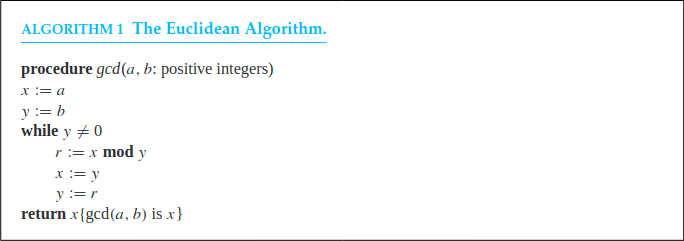
\includegraphics[width=0.7\textwidth]{img-t1/img_850_40.png}
\end{figure}

\textbf{Teorema de Bézout}: sea $a$ y $b$ enteros positivos, $\exists$ enteros $s$ y $t$ tal que gcd(a, b) = $s \cdot a$ + $t \cdot b$ (siendo $s$ y $t$ coeficientes de Bézout).\\
\textbf{Ejemplo}: expresar gcd(252, 198) = 18 como combinación lineal de 252 y 198. \\
252 = 1$\cdot$198 + 54 \\
198 = 3$\cdot$54 + 36 \\
54 = 1$\cdot$36 + 18 \\
36 = 2$\cdot$18 \\

18 = 54 - 1$\cdot$36 (tercera división)\\
36 = 198 - 3$\cdot$54 (segunda división)\\

18 = 54 - 1$\cdot$36 = 54 - 1$\cdot$(198 - 3$\cdot$54) = 3$\cdot$54 - 1$\cdot$198 \\
54 = 252 - 1$\cdot$198 (primera división) \\

resultado: 18 = 4$\cdot$(252 - 1$\cdot$198) - 1$\cdot$198 = \textbf{4}$\cdot$252 \textbf{- 5}$\cdot$198 \\

\textbf{Si $a$, $b$ y $c$ son positivos enteros tal que gcd(a, b) = 1 y $a$ $|$ $bc$, entonces $a$ $|$ $c$.}

\newpage

\section{Arimtética modular}
Si $a$ y $b$ son enteros y $m$ es un positivo entero, entonces $a$ es \textbf{congruente} con $b$ módulo $m$ si $m$ divide a-b ($m$ $|$ $a-b$). Usamos la notación $a \equiv b$ (mod $m$) para indicar lo anterior. Se dice que $a \equiv b$ (mod $m$) es una \textbf{congruencia} y que $m$ es su módulo. \\

\textbf{Sean a y b enteros positivos $a \equiv b$ (mod $m$) entonces $a$ (mod $m$) = $b$ (mod $m$)}. \\
Ejemplo: 34 $\equiv$ 46 (mod 12). 46 mod 12 = 34 mod 12 (10) \\

\textbf{Sea $m$ entero positivo, si $a$ $\equiv$ $b$ (mod $m$) entonces $a$ $\pm$ $c$ $\equiv$ $b$ $\pm$ $d$ (mod $m$)}. \\
Ejemplo: m = 12, a = 13, b = 1, c = 5, d = 17.\\
13 $\equiv$ 25 (mod 12) \\
5 $\equiv$ 17 (mod 12) \\
13 + 5 = 18 y 25 + 17 = 42 \\
18 $\equiv$ 42 (mód 12) \\

\textbf{Sea $m$ un entero positivo y $a$ y $b$ enteros. Entonces \\
($a+b$) mod($m$) = (($a$ mod($m$)) + ($b$ mod($m$))) mod($m$) y \\
$ab$ mod($m$) = (($a$ mod($m$))($b$ mod($m$))) mod ($m$)}. \\
Ejemplo: (25 + 17) mod(12) = (25 mod (12) + 17 mod(12)) mod(12) = (1 + 5)mod(12) = 6 

\subsection{Aritmética módulo m}
Por una parte: $a_m$ + $b$ := (a + b) mod(m), y por otra: $a_m$ $\cdot$ $b$ := (a $\cdot$ b) mod(m). \\
\textbf{Los “números buenos” o unidades de $Z_m$ son primos relativos con $m$}, el resto son “malos”. En $Z_m$ hay $p$ - 1 unidades (todos menos el 0) si $m$ es primo y $\varPhi (m)$ si no lo es, las unidades son los elementos que tienen inverso multiplicativo. ($a$ es una unidad si $\exists$ un $b$ tal que $a$ $\cdot$ $b$ = 1, siendo así $a$ inversible). \\
$m$ = $p^k$, y $\varPhi (p^k) = p^{k-1}(p-1)$ \\

\textbf{Teorema fundamental de la aritmética}:  $m$ = $p_1^{\alpha 1}$ $\cdot$ $p_2^{\alpha 2}$ $\cdot$ ... $\cdot$ $p_s^{\alpha s}$ ($p_i$ primos diferentes). \\
$\varPhi (m)$ = $\varPhi (p_1^{\alpha 1})$ $\cdot$ $\varPhi (p_2^{\alpha 2})$ $\cdot$ ... $\cdot$ $\varPhi (p_s^{\alpha s})$ \\
$\varPhi_{12}$ = $\varPhi (2^2)$ $\cdot$ $\varPhi (3)$ = $2^{2-1} \cdot (2-1) \cdot 3^{1-1} \cdot (3-1)$ = $2 \cdot 2$ = 4. (12 = $2^2 \cdot 3$) En $Z_{12}$ hay 4 números buenos. 

\subsection{Congruencias lineales}
Sea $ax$ $\equiv$ $b$ mod($m$): \\
$d$ = gcd($a$, $m$) $\not|$ $b$ (\textbf{no tiene solución}): 2x $\equiv$ 3 mod(6), gcd(2, 6) = 2 $\not|$ 3. \\
$d$ = gcd($a$, $m$) $|$ $b$ (\textbf{tiene d soluciones}): 2x $\equiv$ 4 mod(6), gcd(2, 6) = 2 $|$ 4. \\
$\frac{a}{d}x \equiv \frac{b}{d} mod(\frac{m}{d})$ (\textbf{tiene una única solución $x_0$}): 237x $\equiv$ 4 mod(491), gcd(237, 491) = 1 = $s \cdot 237 + t \cdot 491. 4 = 4s \cdot 237 + 4t \cdot 491$. (gcd($\frac{a}{d}$, $\frac{m}{d}$) = 1). 

\subsection{Pequeño teorema de Fermat}
Si $p$ es primo y $p \not| a$, entonces $a^{p-1} \equiv 1 mod(p)$. \\
Ejemplo: 13 $\not|$ 237 (p = 13, a = 237). $237^{13-1} = 237^12 = 1 mod(13)$

\subsection{Euler}
\textbf{Sea m primo, si gcd(a, m) = 1, entonces $a^{\varPhi (m)} \equiv 1 mod(m)$.} \\
gcd(a, p) = 1 $\Leftrightarrow$ $p \not| a$ \\
$\varPhi (p) \equiv 1 mod(p)$ \\
$\varPhi (p) = p - 1$.

\newpage

\subsection{Teorema chino de los restos}
Sean $m_1$, $m_2$, ..., $m_n$ primos relativos entre ellos. Sean $a_1$, $a_2$, ..., $a_k$ enteros. Entonces el sistema (el de abajo) tiene una única solución módulo m = $m_1 \cdot m_2 \cdot m_3 \cdot ... \cdot m_n$ ($0 \leq x < m$) 


$$\begin{cases} x \equiv a_1 \mod m_1 \\
x \equiv a_2 \mod m_2 \\
... \\
x \equiv a_k \mod m_k \end{cases}$$

x = $a_1 \cdot \frac{m}{m_1} \cdot [\frac{m}{m_1}]^{-1}_{m_1} + a_2 \cdot \frac{m}{m_2} \cdot [\frac{m}{m_2}]^{-1}_{m_2} + ... + a_k \cdot \frac{m}{m_k} \cdot [\frac{m}{m_k}]^{-1}_{m_k}$ \\

Ejemplo: $$\begin{cases} x \equiv 2 \mod 3 \\
x \equiv 3 \mod 5 \\
x \equiv 2 \mod 7 \end{cases}$$

x = $2 \cdot \frac{105}{3} \cdot [\frac{105}{3}]^{-1}_3 + 3 \cdot \frac{105}{5} \cdot [\frac{105}{5}]^{-1}_5 + 2 \cdot \frac{105}{7} \cdot [\frac{105}{7}]^{-1}_7$ \\

x = $2 \cdot 35 \cdot [35]^{-1}_3 + 3 \cdot 21 \cdot [21]^{-1}_5 + 2 \cdot 15 \cdot [15]^{-1}_7$ = $2 \cdot 35 \cdot 2 + 3 \cdot 21 \cdot 1 + 2 \cdot 1$ = $233$ \\

$233 \equiv 23 \mod 105$

\section{Criptografía}
Disciplina que trata el estudio de códigos cifrados. Existen diferentes tipos de sistemas criptográficos: 
\begin{itemize}
    \item \textbf{Cifrado de clave simétrica} (una única clave privada): dentro de esta categoría existen: cifrado por sustitución (reemplaza un carácter por otro) o el cifrado por traslación (desplaza el alfabeto un número de posiciones). En este último tipo de cifrado se encuentra el \textbf{cifrado César}, donde cada letra del texto se desplaza un número fijo de posiciones en el alfabeto. Por ejemplo, con un desplazamiento de 3, la letra A se convierte en D.

    \item \textbf{Cifrado de clave asimétrica} (dos claves diferentes): se usan funciones unidireccionales, dónde un sentido de la transmisión es fácil, pero el contrario es difícil. Se emplea una clave pública para cifrar el mensaje y se descifra con la clave privada que tiene el receptor. Multiplicamos 2 primos, p y q, dando n, que es muy fácil de obtener, pero es difícil de factorizar para conseguir p y q. Esta es la base del \textbf{RSA}.
\end{itemize}

\newpage

\subsection{RSA}
El cifrado RSA se basa en la dificultad de factorizar un número grande. Para ello, se eligen dos números primos grandes, $ p $ y $ q $. A partir de estos, se calcula $ n $ como:

$$n = p \cdot q$$

Luego, se calcula la función $\varPhi$ de Euler $ \varPhi(n) $:

$$\varPhi(n) = \varPhi(p) \cdot \varPhi(q) = (p-1) \cdot (q-1)$$

A continuación, se elige un número $ e $ tal que $ 1 < e < \varPhi(n) $ y que sea coprimo con $ \varPhi(n) $. Esto significa que $ \gcd(e, \varPhi(n)) = 1 $. El número $ e $ debe tener un inverso multiplicativo $ d $ tal que:

$$d \cdot e \equiv 1 \mod \varPhi(n)$$

Esto implica que $ d $ es el inverso multiplicativo de $ e $ módulo $ \varPhi(n) $.


Para cifrar un mensaje $ m $, se utiliza la siguiente fórmula:

$$E(m) \equiv m^e \mod n$$

Donde $ E(m) $ es el mensaje cifrado. Para descifrar el mensaje, se aplica la siguiente operación:

$$D(c) \equiv c^d \mod n$$

Donde $ c $ es el mensaje cifrado. Al aplicar el descifrado al mensaje cifrado, se obtiene:

$$D(E(m)) = E(m)^d = (m^e)^d \equiv m \mod n$$

Esto demuestra que el proceso de cifrado y descifrado es correcto, ya que se recupera el mensaje original $ m $. \\

\textbf{Ejemplo}:

Supongamos que elegimos los primos $ p = 61 $ y $ q = 53 $.

Calculamos $ n $ y $ \varPhi(n) $:

$$n = 61 \cdot 53 = 3233$$
$$\varPhi(n) = (61-1)(53-1) = 60 \cdot 52 = 3120$$

Elegimos $ e = 17 $ (que es coprimo con 3120). Ahora, encontramos $ d $ tal que:

$$d \cdot 17 \equiv 1 \mod 3120$$

Usando el algoritmo extendido de Euclides, encontramos que $ d = 2753 $.

Ahora, ciframos un mensaje $ m = 123 $:

$$E(m) \equiv 123^{17} \mod 3233$$

Calculando $ E(m) $:

$$E(123) \equiv 855 \mod 3233$$

Para descifrar, aplicamos:

$$D(c) \equiv 855^{2753} \mod 3233$$

Calculando $ D(855) $:

$$D(855) \equiv 123 \mod 3233$$

Así, hemos cifrado y descifrado correctamente el mensaje original.

\section{Representación de $n$ en base $>$ 1 (expansión)}

Sea $ b $ un entero mayor que 1. Si $ a $ es un entero positivo, entonces un número $ n $ se puede expresar de manera única en la forma:

$$n = (a_k \cdot b^k + a_{k-1} \cdot b^{k-1} + \ldots + a_1 \cdot b^1 + a_0 \cdot b^0)$$

donde $ k $ es un entero no negativo, $ 0 \leq a_0, a_1, \ldots, a_k < b $ y $ a_k \neq 0 $.


\begin{itemize}
    \item $ b = 2 $ (Binario): $15_{10} = 1111_2$
    \item $ b = 8 $ (Octal): $14_{10} =  2371_8$
\end{itemize}


Para convertir un número de decimal a una base $ b $, se sigue el siguiente procedimiento: 
\begin{enumerate}
    \item Dividir el número entre $ b $.
    \item Anotar el resto.
    \item Repetir el proceso con el cociente hasta que este sea 0.
    \item Los restos anotados, leídos en orden inverso, representan el número en la base $ b $.
\end{enumerate}

\textbf{Ejemplo}: \\
Supongamos que queremos convertir el número decimal $ n = 100 $ a base $ 7 $.

\begin{enumerate}
    \item $ 101 \div 7 = 14 $ con un resto de $ 3 $.
    \item $ 14 \div 7 = 2 $ con un resto de $ 0 $.
    \item $ 2 \div 7 = 0 $ con un resto de $ 2 $.
\end{enumerate}

Ahora, leemos los restos en orden inverso: $ 2, 0, 3 $.

Por lo tanto, el número $ 101 $ en base $ 7 $ se representa como:

$$(203)_7$$

\newpage

\section{Criterios de divisibilidad}

Los criterios de divisibilidad son reglas que permiten determinar si un número es divisible por otro sin necesidad de realizar la división completa. A continuación se presentan algunos de los criterios más comunes:

\begin{itemize}
    \item \textbf{Divisibilidad por 2:} 
    $$n = 2 \quad \Rightarrow \quad \text{El número es par.}$$
    Un número es divisible por 2 si su última cifra es par (0, 2, 4, 6, 8).

    \item \textbf{Divisibilidad por 3:} 
    $$n = 3 \quad \Rightarrow \quad 3 \mid S \quad \text{(donde $ S $ es la suma de las cifras del número).}$$
    Un número es divisible por 3 si la suma de sus cifras es divisible por 3.

    \item \textbf{Divisibilidad por 4:} 
    $$n = 4 \quad \Rightarrow \quad 4 \mid (2 \cdot a_1 + a_0)$$
    Un número es divisible por 4 si los dos últimos dígitos forman un número que es divisible por 4.

    \item \textbf{Divisibilidad por 5:} 
    $$n = 5 \quad \Rightarrow \quad a_0 = 0 \quad \text{o} \quad 5$$
    Un número es divisible por 5 si su última cifra es 0 o 5.

    \item \textbf{Divisibilidad por 6:} 
    $$n = 6 \quad \Rightarrow \quad \text{Divisible por 2 y 3.}$$
    Un número es divisible por 6 si es divisible por 2 y por 3.

    \item \textbf{Divisibilidad por 7:} 
    $$n = 7 \quad \Rightarrow \quad a_k \cdot a_{k-1} \cdots a_1 - 2 \cdot a_0$$
    Se toma el número formado por todas las cifras menos la última, se le resta el doble de la última cifra, y si el resultado es divisible por 7, entonces el número original también lo es.

    \item \textbf{Divisibilidad por 8:} 
    $$n = 8 \quad \Rightarrow \quad 2 \mid a_2 a_1 a_0$$
    Un número es divisible por 8 si los últimos tres dígitos forman un número que es divisible por 8.

    \item \textbf{Divisibilidad por 9:} 
    $$n = 9 \quad \Rightarrow \quad 9 \mid S \quad \text{(donde $ S $ es la suma de las cifras del número).}$$
    Un número es divisible por 9 si la suma de sus cifras es divisible por 9.

    \item \textbf{Divisibilidad por 10:} 
    $$n = 10 \quad \Rightarrow \quad a_0 = 0$$
    Un número es divisible por 10 si su última cifra es 0.

    \item \textbf{Divisibilidad por 11:} 
    $$n = 11 \quad \Rightarrow \quad 11 \mid (S_p - S_i)$$
    Donde $ S_p $ es la suma de las cifras en las posiciones pares y $ S_i $ es la suma de las cifras en las posiciones impares. Un número es divisible por 11 si la diferencia entre estas dos sumas es divisible por 11.
\end{itemize}





\begin{comment}
\begin{figure}[h]
    \centering
    \includegraphics[width=0.65\textwidth]{1.png}
    \caption{}
\end{figure}
\end{comment}

\begin{comment}
\begin{wrapfigure}[]{r}{0.45\linewidth}
    \centering
    \includegraphics[width=0.8\linewidth]{8.png}
    \caption{}
\end{wrapfigure}
\end{comment}

\end{document}